\documentclass[11pt,a4paper]{article}

% Required packages
\usepackage[utf8]{inputenc}
\usepackage[T1]{fontenc}
\usepackage{times} % Times New Roman font
\usepackage{CJK} % For Japanese text support
\usepackage{geometry}
\usepackage{multicol}
\usepackage{setspace}
\usepackage{graphicx}
\usepackage{svg}
\usepackage{xcolor}
\usepackage{fancyhdr}
\usepackage{titlesec}
\usepackage{caption}     % For \captionof

% Page geometry setup
\geometry{
    a4paper,
    top=25mm,
    bottom=30mm,
    left=18mm,
    right=18mm
}

% Remove page numbers
\pagestyle{empty}
% Remove spacing before and after section titles
\titlespacing*{\section}{0pt}{0pt}{0pt}
\titlespacing*{\subsection}{0pt}{0pt}{0pt}

% Configure two-column layout
% Column width: 83.5mm each, spacing: 7mm
\setlength{\columnsep}{7mm}
\setlength{\columnwidth}{83.5mm}

% Configure section titles (chapter titles)
\titleformat{\section}
{\normalfont\fontsize{12}{12}\bfseries}{\thesection}{1em}{}

\titleformat{\subsection}
{\normalfont\fontsize{11}{11}\bfseries}{\thesubsection}{1em}{}

% Line spacing to achieve approximately 60 lines per column
\linespread{1.0}

% Remove paragraph indentation and add spacing
\setlength{\parindent}{0pt}
\setlength{\parskip}{0.5ex}

% Control word spacing
\spaceskip=0pt






\begin{document}
% First page header setup (6 lines from top)
\begin{center}
% Line 1: blank
~\\
% Line 2: Title in English (Times New Roman, 12pt, Center)
% {\fontsize{12}{14}\selectfont \textbf{A Multifaceted Exploration of Spatial Openness in Rental Housing: Big Data Analysis Across Tokyo's 23 Wards}}\\
{\fontsize{12}{14}\selectfont \spaceskip=0pt plus 1fil \textbf{Multifaceted Exploration of Spatial Openness in Rental Housing: A Big Data Analysis in Tokyo's 23 Wards}}\\

% Line 3: Title in Japanese (Noto Sans CJK, 11pt, Center, Bold)
\begin{CJK}{UTF8}{min}
{\fontsize{11}{11}\selectfont {賃貸住宅における空間開放性の多面的探究:東京23区のビッグデータ分析}}
\end{CJK}\\
% Line 4: blank
\end{center}
% Line 5: Affiliation, Student ID, Name (Times New Roman, 11pt, Right-justified)
\begin{flushright}
{\fontsize{11}{13}\selectfont \spaceskip=0pt OKI Lab  23M58033 \begin{CJK}{UTF8}{min}リュ ゲン\end{CJK} (Liu Yuan)}
\end{flushright}
% Line 6: blank
%\vspace{0.1mm}
% Main body starts from line 7
\begin{multicols}{2}
\fontsize{11}{13}\selectfont
\spaceskip=0pt
\vspace{1em}

\section{Introduction}

Spatial openness encompasses perceived spaciousness, visual connectivity, and 
flow within living environments. Traditional approaches using floor area and room count 
fail to capture nuanced spatial qualities from interior imagery and floor plans.
This research proposes a methodology integrating interior images with semantic 
segmentation and visibility graph analysis to quantify spatial openness in rental housing. 
We analyze distributions across Tokyo's 23 wards and construction decades, investigating correlations with subjective impression scores.
Our approach enables automated spatial quality analysis, opening possibilities for large-scale urban studies of residential design.


\vspace{1em}

\section{Openness Attributes Extraction}

\subsection{Dataset and Attributes}

Our dataset comprises a few thousand rental properties from Tokyo's 23 wards (1960-present), 
sampled to ensure each decade has roughly equal data and filtered for image quality and data completeness. The data selection process is
shown as Figure \ref{fig:data_selection}.
\begin{center}
    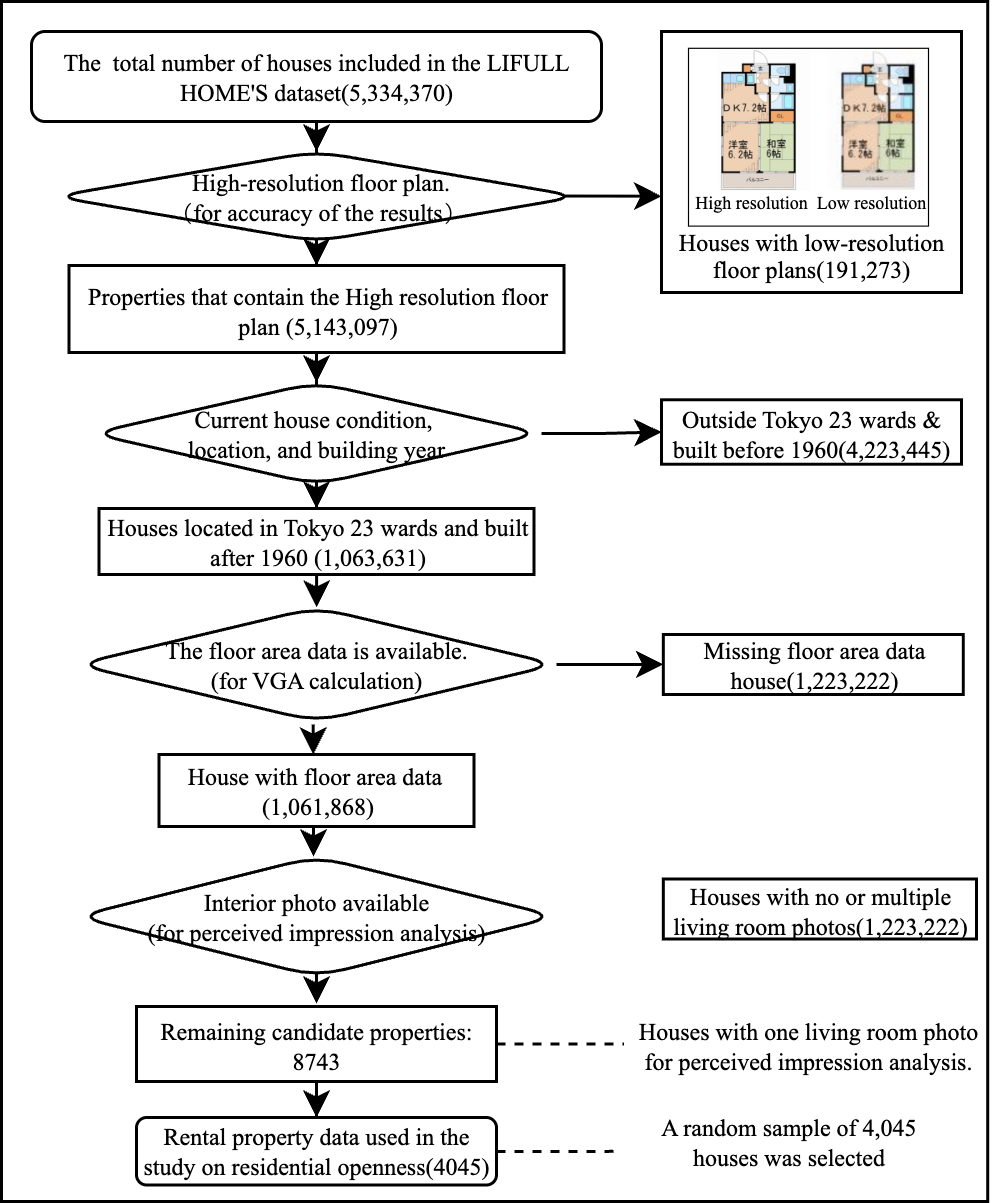
\includegraphics[width=0.95\columnwidth]{plots/data_filtering.png}
    \captionof{figure}{Data selection and filtering process.}
    \label{fig:data_selection}
\end{center}



As illustrated in Figure \ref{fig:overview_02}, this overview shows our methodology extracts multiple categories of spatial openness 
attributes through 3D interior images, 2D floorplan data, and property specifications, as well as our following data analysis. 
\begin{center}
    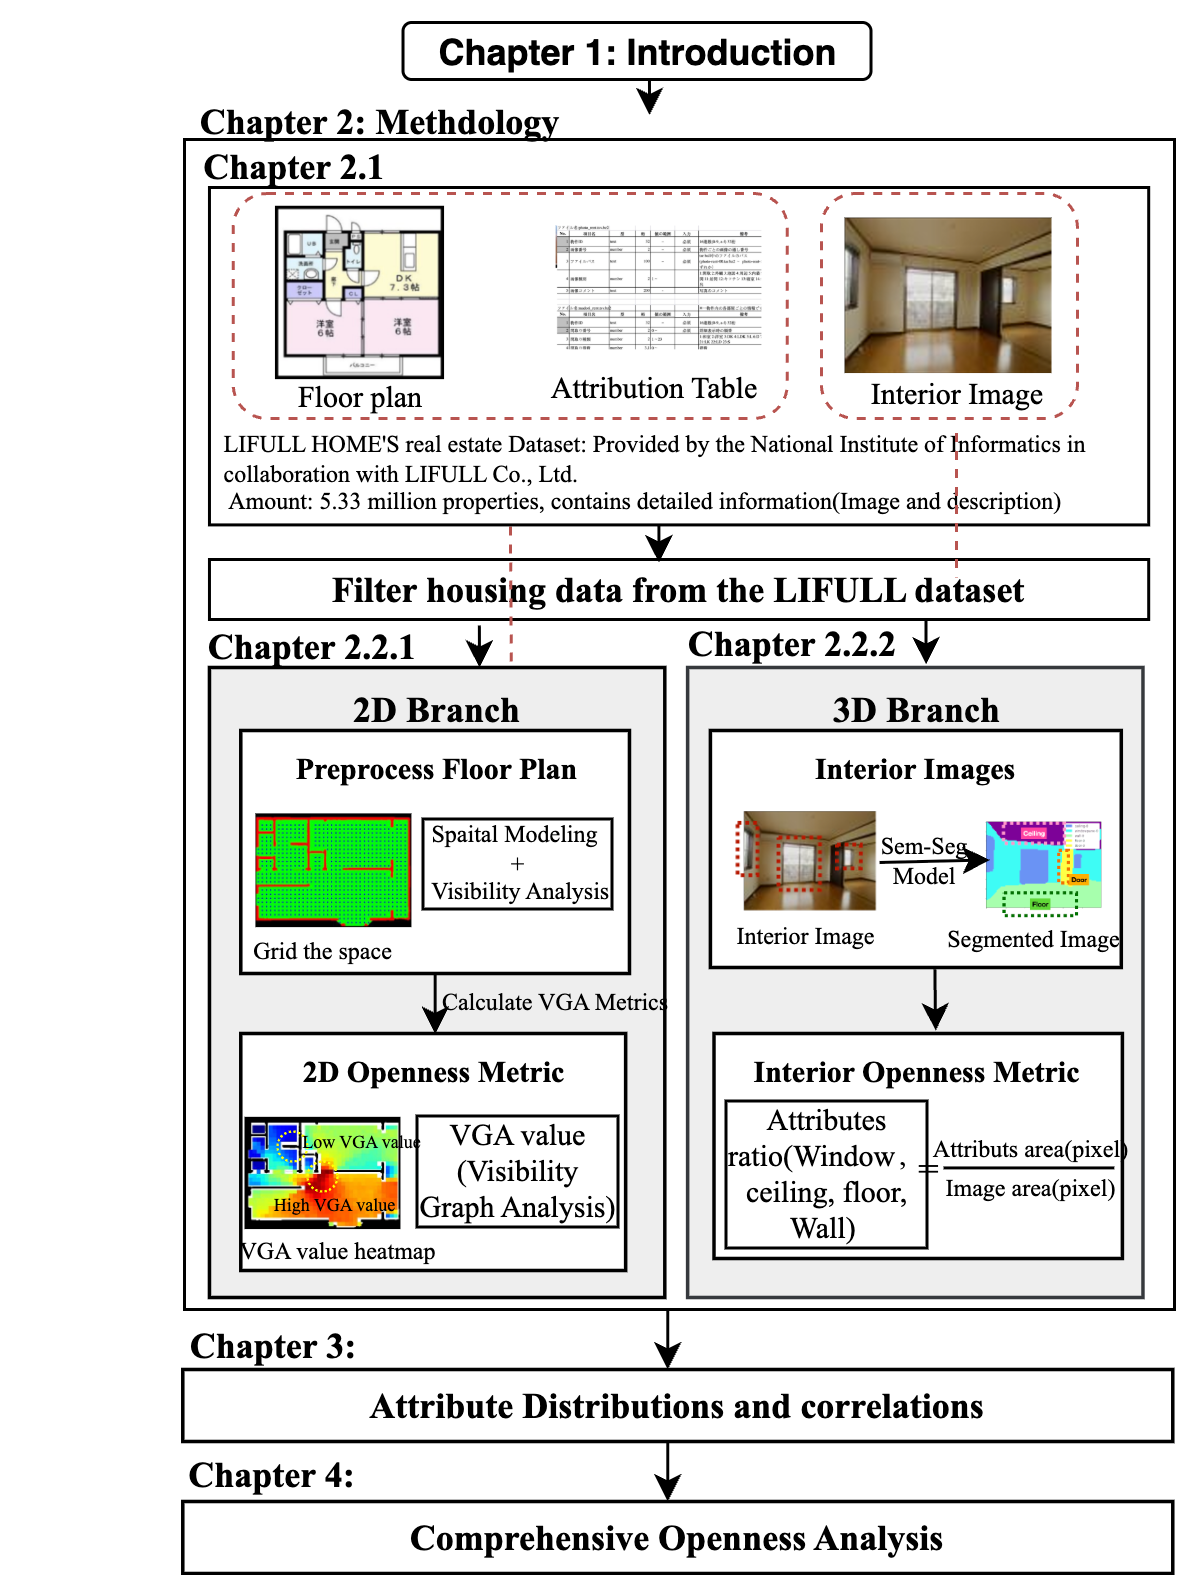
\includegraphics[width=0.95\columnwidth]{plots/overview.png}
    \captionof{figure}{Feature extraction overview.}
    \label{fig:overview_02}
\end{center}
Impression scores (Q3) are extracted using Shimomura et al.'s pre-trained model.
The following attributes are the focus of our analysis:
\textbf{room size attributes}, \textbf{property specifications}, \textbf{interior elements}, and \textbf{vga-based statistics}.
Room size attributes and property specifications are obtained directly from the database.
Interior elements are extracted through semantic segmentation of interior images, 
while VGA-based statistics are computed from floorplan analysis to quantify spatial connectivity. 

\subsection{Interior Elements}
We apply Mask2Former semantic segmentation to extract wall, ceiling, floor, and window ratios from interior images. 
The fractions of each visual element are calculated by the fraction of pixels from the segmentation mask.



\subsection{VGA-based Statistics}
For floorplan data, we use semantic segmentation to identify walls, rooms, and open areas. 
We then create a grid over the open areas and calculate VGA (Visibility Graph Analysis) values:
\begin{equation}
\label{eq:vga_definition}
S(i) = \sum_{j=1}^{N} V_{ij}
\end{equation}
where $S(i)$ is the visibility score at node $i$, and $V_{ij} = 1$ if node $j$ is visible from node $i$, otherwise $V_{ij} = 0$. 
This creates a VGA heatmap showing spatial connectivity throughout the floorplan. We extract summary statistics 
(mean, standard deviation, percentiles) from this heatmap as spatial openness features, as shown in Figure \ref{fig:madori_processing}.
After extracting the statistics, we can utilize them to analyze their distributions and correlations with other attributes to enhance the understanding of spatial openness.
of the openness of the properties.

\begin{center}
    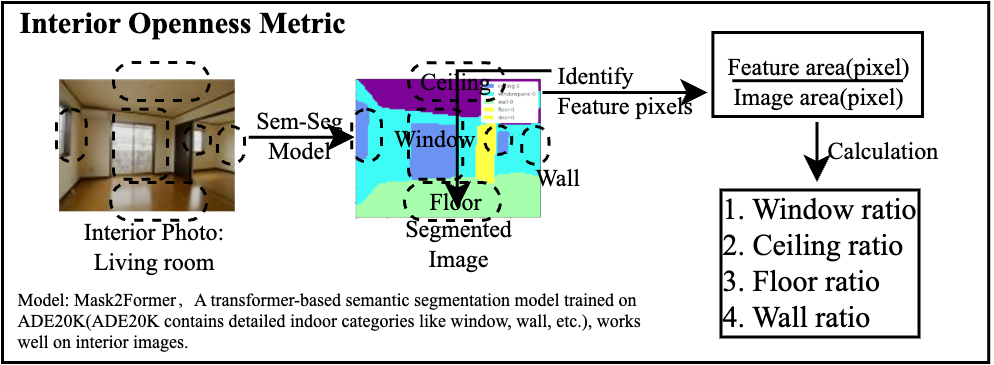
\includegraphics[width=0.99\columnwidth]{plots/exp_lv_semseg_5.png}
    % \\[0.5em]
    % 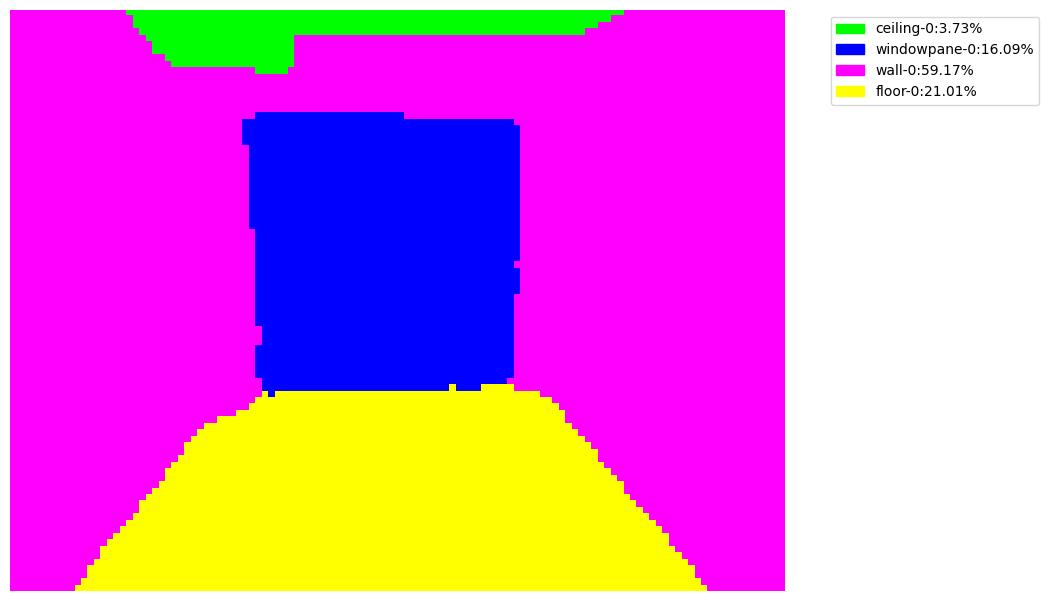
\includegraphics[width=\columnwidth]{plots/exp_lv_semseg_1.jpg}
    \captionof{figure}{Interior semantic segmentation and impression scoring.}
    \label{fig:interior_semseg}
\end{center}

\vspace{1em}

\section{Attribute Distributions and Correlations}

\subsection{Temporal Analysis of Spatial Openness}
From the tabular features of the properties, we have various information, with the most interesting 
being building age and geographic factors. 
We examined the distribution of VGA mean values across construction dates in decades, as shown in 
Figure \ref{fig:temporal_analysis}.

The analysis shows VGA mean values contain large outliers but remain stable across decades, likely due to large-area properties. 
The impression scores show more balanced distributions, as they are evaluated from interior images that are less dependent of overall property layouts.
\begin{center}
    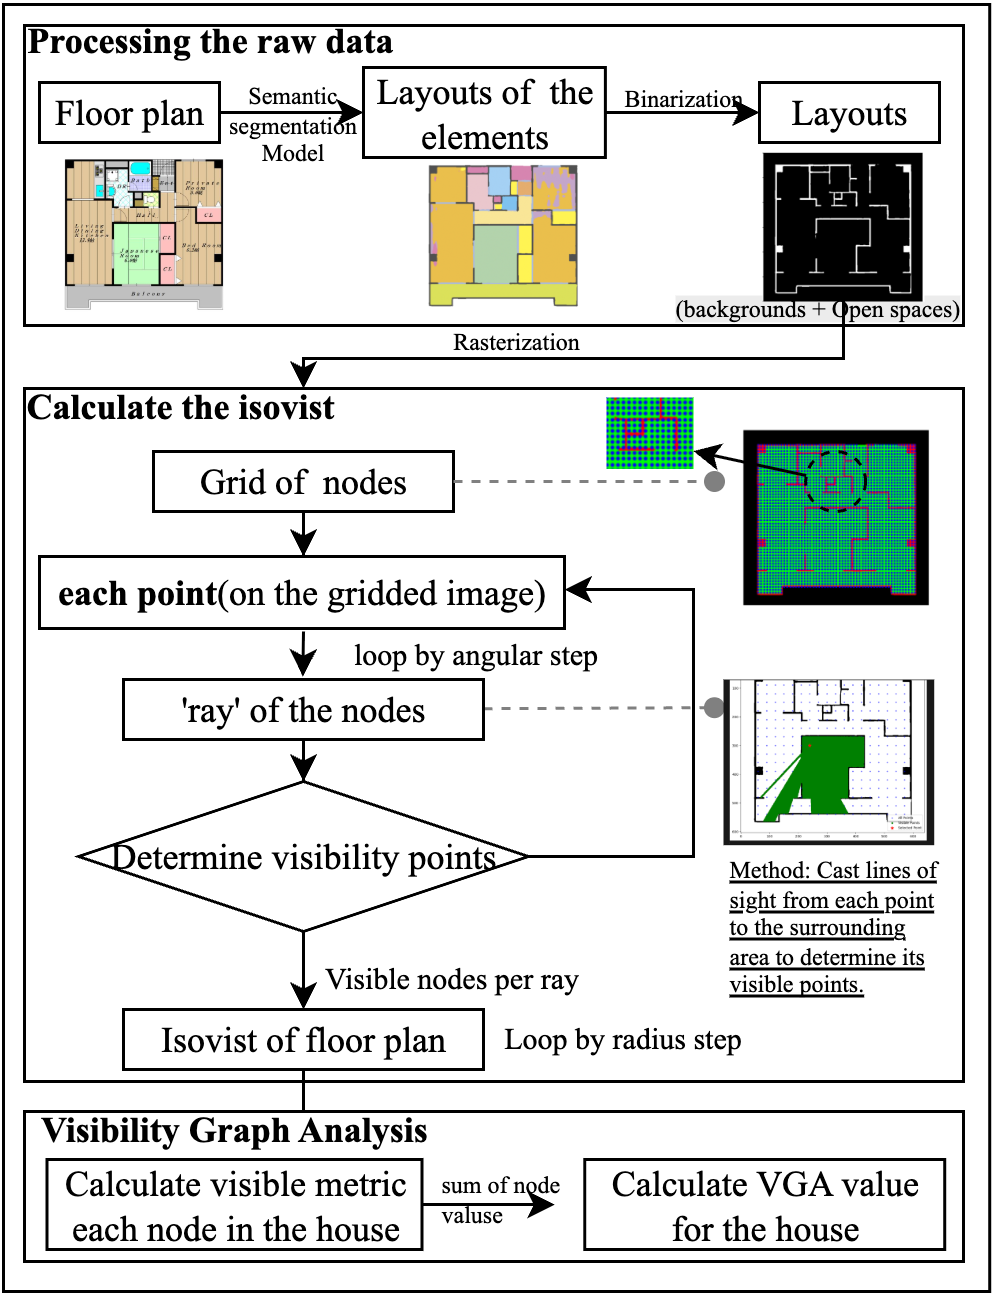
\includegraphics[width=0.95\columnwidth]{plots/vga_process.png}
    \captionof{figure}{Workflow of creating VGA heatmap from floorplan data: raw floorplan, semantic segmentation output, physical gridding, and VGA heatmap.}
    \label{fig:madori_processing}
\end{center}

\begin{center}
    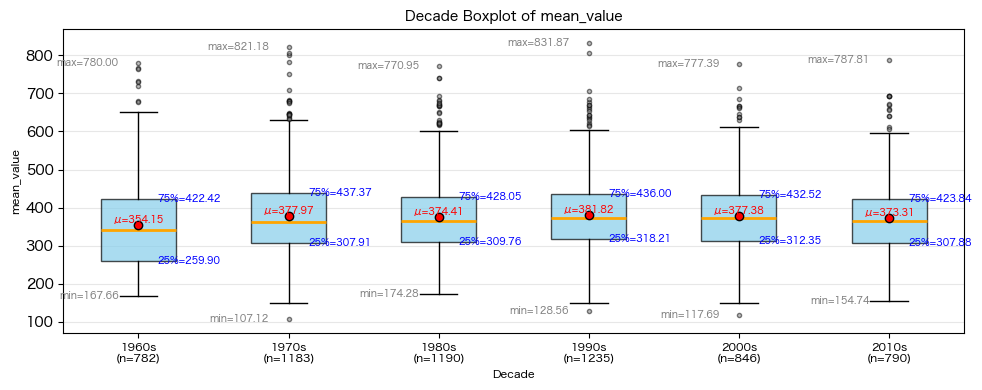
\includegraphics[width=0.9\columnwidth]{plots/vga_10years_box.png}
    \captionof{figure}{Distribution of VGA mean values across construction dates by decade}
    \label{fig:temporal_analysis}
\end{center}
\subsection{Geographic Distribution Analysis}

We conducted a comprehensive analysis of the geographic distribution of VGA mean values and impression scores at the chome-level granularity using post-code alignment across Tokyo's 23 special wards, as shown in Figure \ref{fig:geo_analysis}. This fine-grained spatial analysis allows us to examine potential neighborhood-level variations in spatial openness characteristics. However, despite this detailed geographic examination, no clear clustering patterns or significant imbalances are found in the distributions across the different areas for either attribute, suggesting that spatial openness characteristics are relatively uniformly distributed across Tokyo's urban landscape.

\subsection{Correlation Analysis Between Openness Attributes}
We conducted a detailed correlation analysis examining the relationships between VGA statistics, impression scores, and interior element fractions to understand how different measures of spatial openness relate to each other.
Figure \ref{fig:corr_vga_q3} reveals only mild correlations between VGA metrics derived from floorplan analysis and impression scores obtained from interior imagery assessment, suggesting fundamental gaps between objective floorplan-based spatial analysis and subjective imagery-based perceptual assessment of spatial openness.
\vspace{1em}

\section{Comprehensive Openness Analysis}
\subsection{Analysis of Impression Scores and Interior Elements}
We performed core-component dependency analysis combining impression scores 
with interior element ratios after applying rigorous outlier filtering using a 75th percentile cutoff to ensure data quality. The cluster analysis reveals distinct 
groupings based on floor and ceiling visibility characteristics, with moderate negative correlations observed with impression scores, indicating that higher visibility of structural elements tends to correspond with lower perceived spatial openness, 
as demonstrated in Figure \ref{fig:inter_q3_cluster} and quantified in Table \ref{tab:interior_corr}.

\begin{center}
    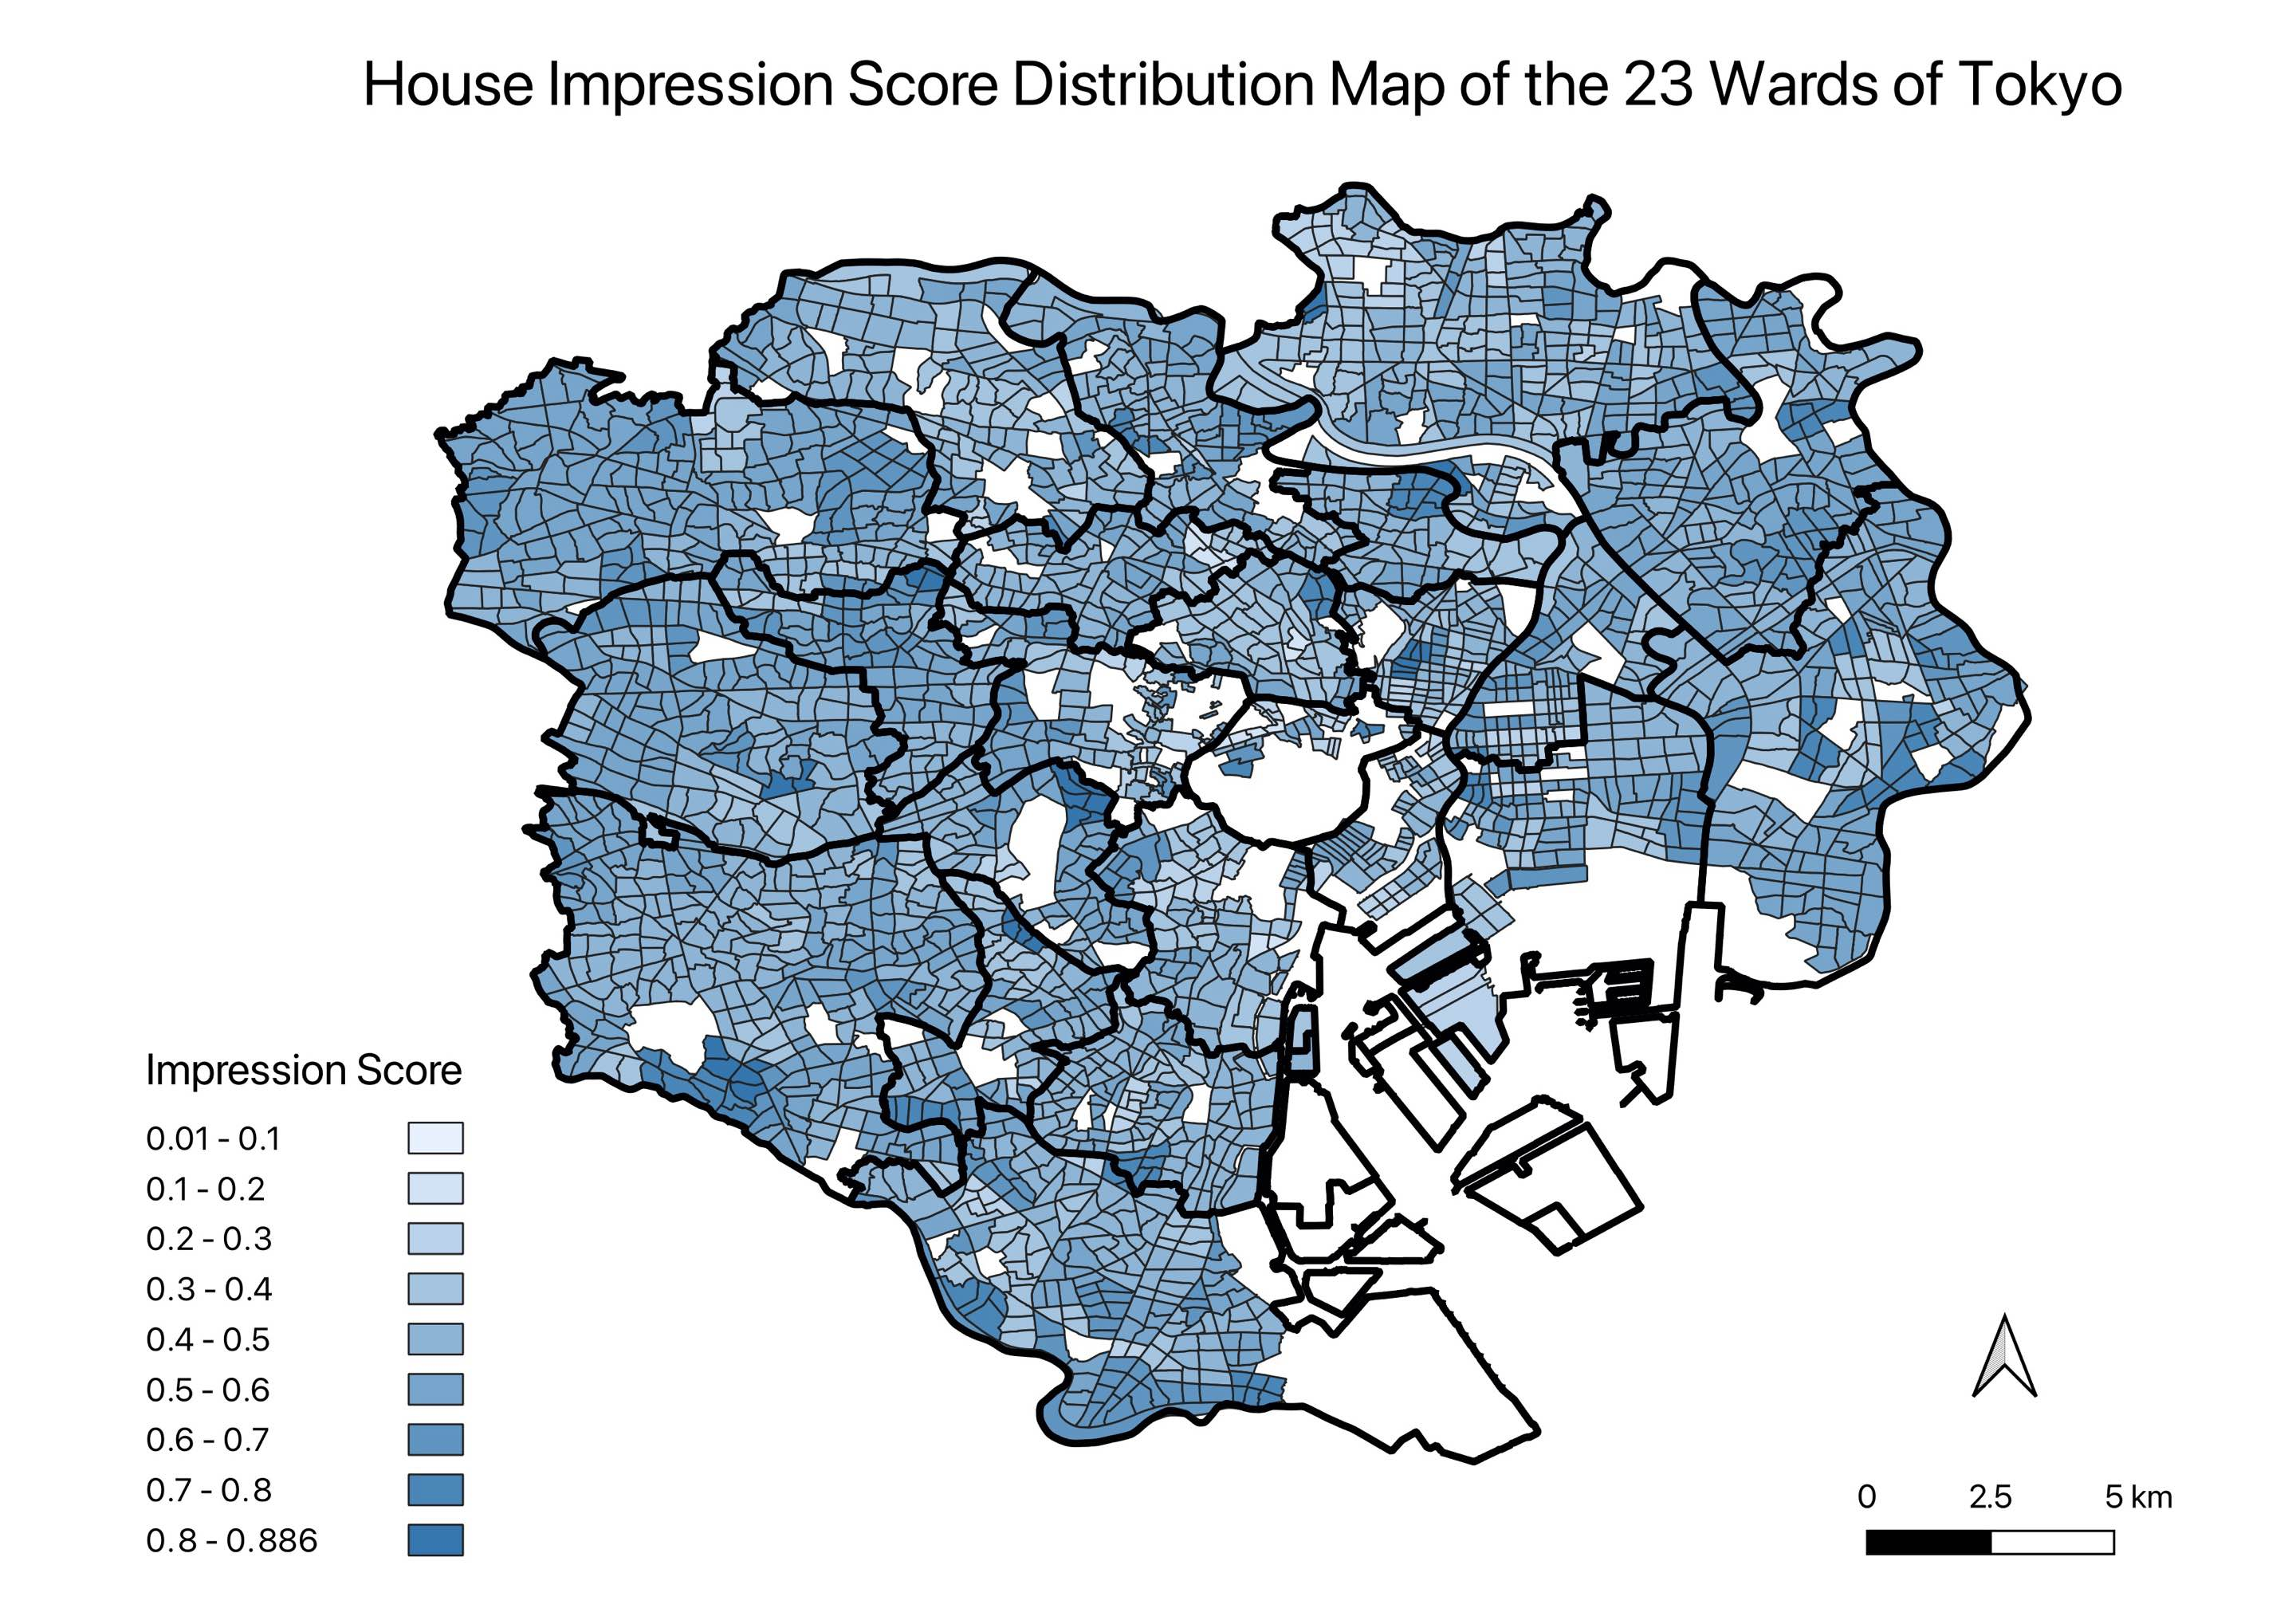
\includegraphics[width=0.8\columnwidth]{plots/tokyo23_q3_geo.jpg}
    \\[0.5em]
    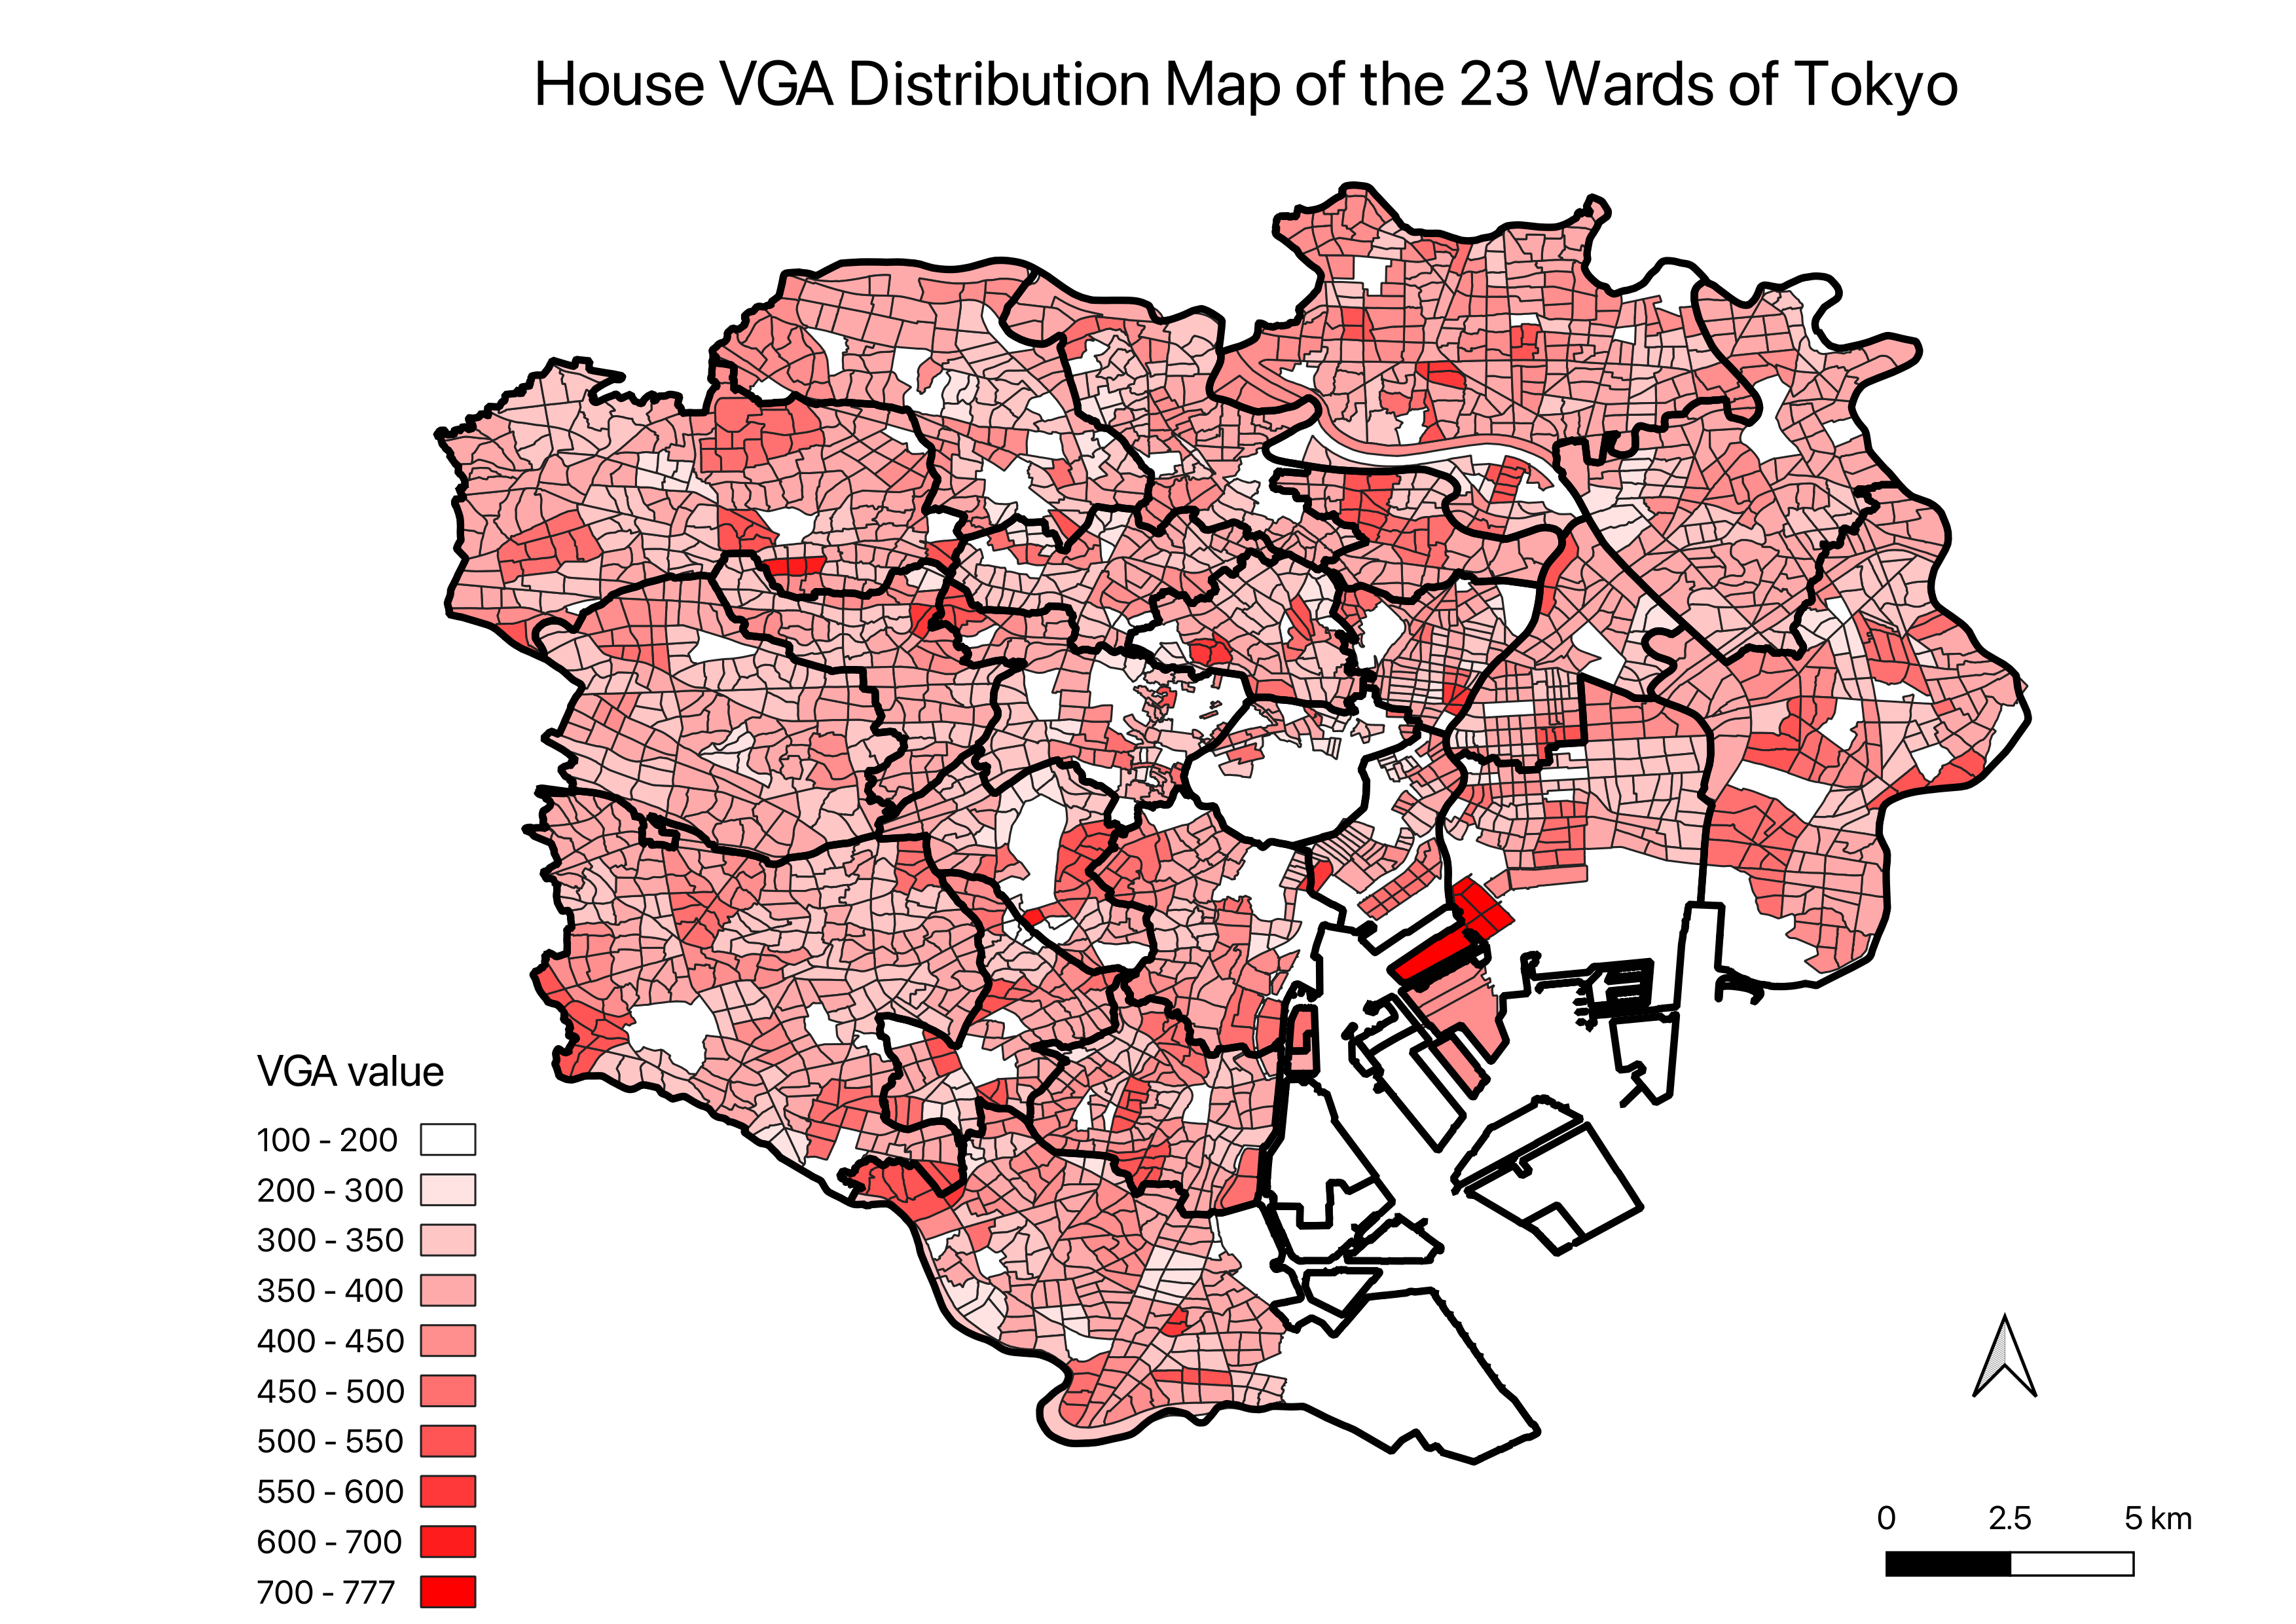
\includegraphics[width=0.8\columnwidth]{plots/tokyo23_vga_geo.png}
    \captionof{figure}{Geographic distribution analysis across Tokyo's 23 special wards: impression scores (top) and VGA mean values (bottom).}
    \label{fig:geo_analysis}
\end{center}

\begin{center}
    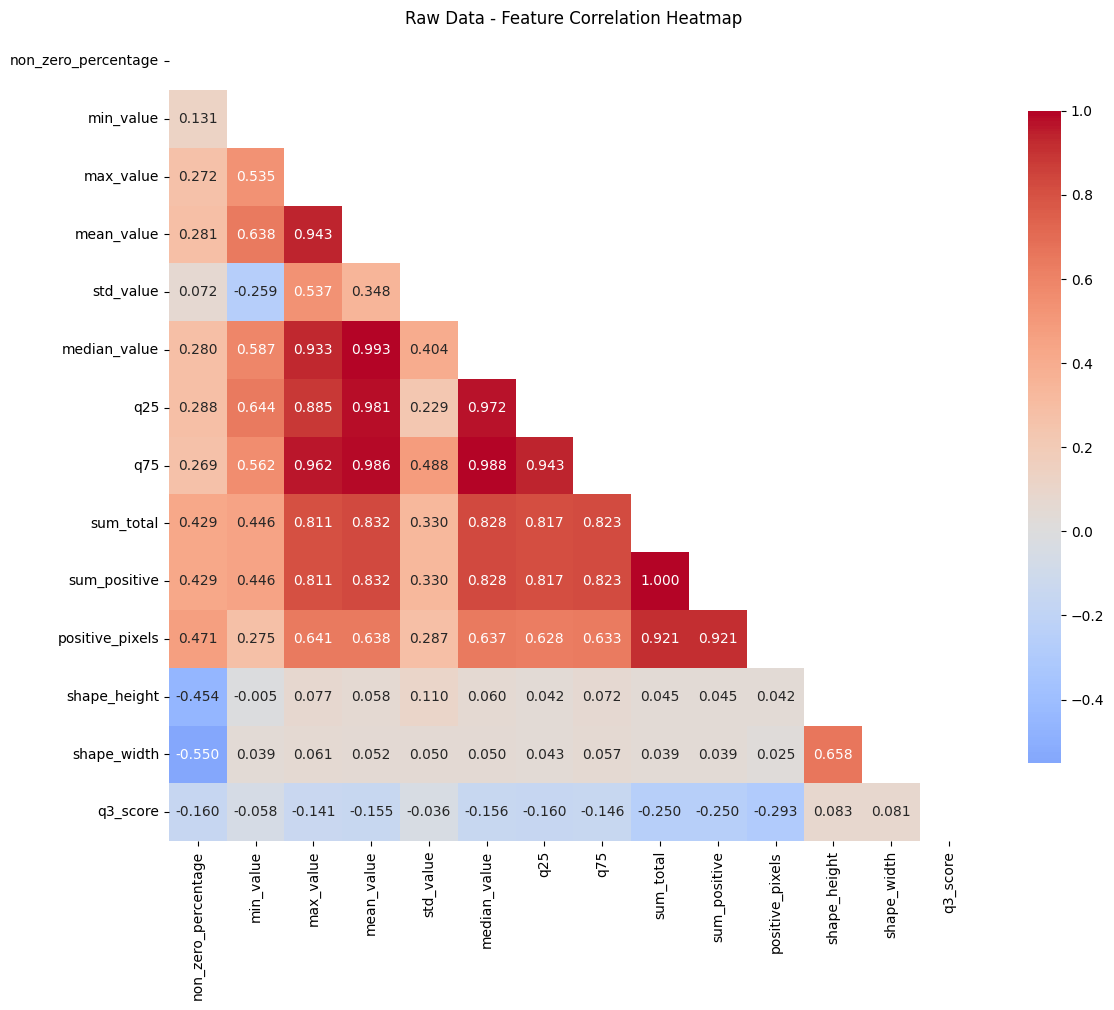
\includegraphics[width=0.8\columnwidth]{plots/corr_vga_q3.png}
    \captionof{figure}{Correlation matrix between Q3 impression scores, VGA metrics (mean, std, min, max), and interior element fractions}
    \label{fig:corr_vga_q3}
\end{center}


\begin{center}
\begin{tabular}{lcc}
\hline
Interior Element & Correlation & Sample Size (n) \\
\hline
Windowpane & 0.0905 & 3012 \\
Floor & -0.1577 & 4439 \\
Ceiling & -0.3043 & 3559 \\
Wall & 0.0275 & 4430 \\
\hline
\end{tabular}
\captionof{table}{Correlations between interior element ratios and Q3 impression scores after 75\% filtering}
\label{tab:interior_corr}
\end{center}

\begin{center}
    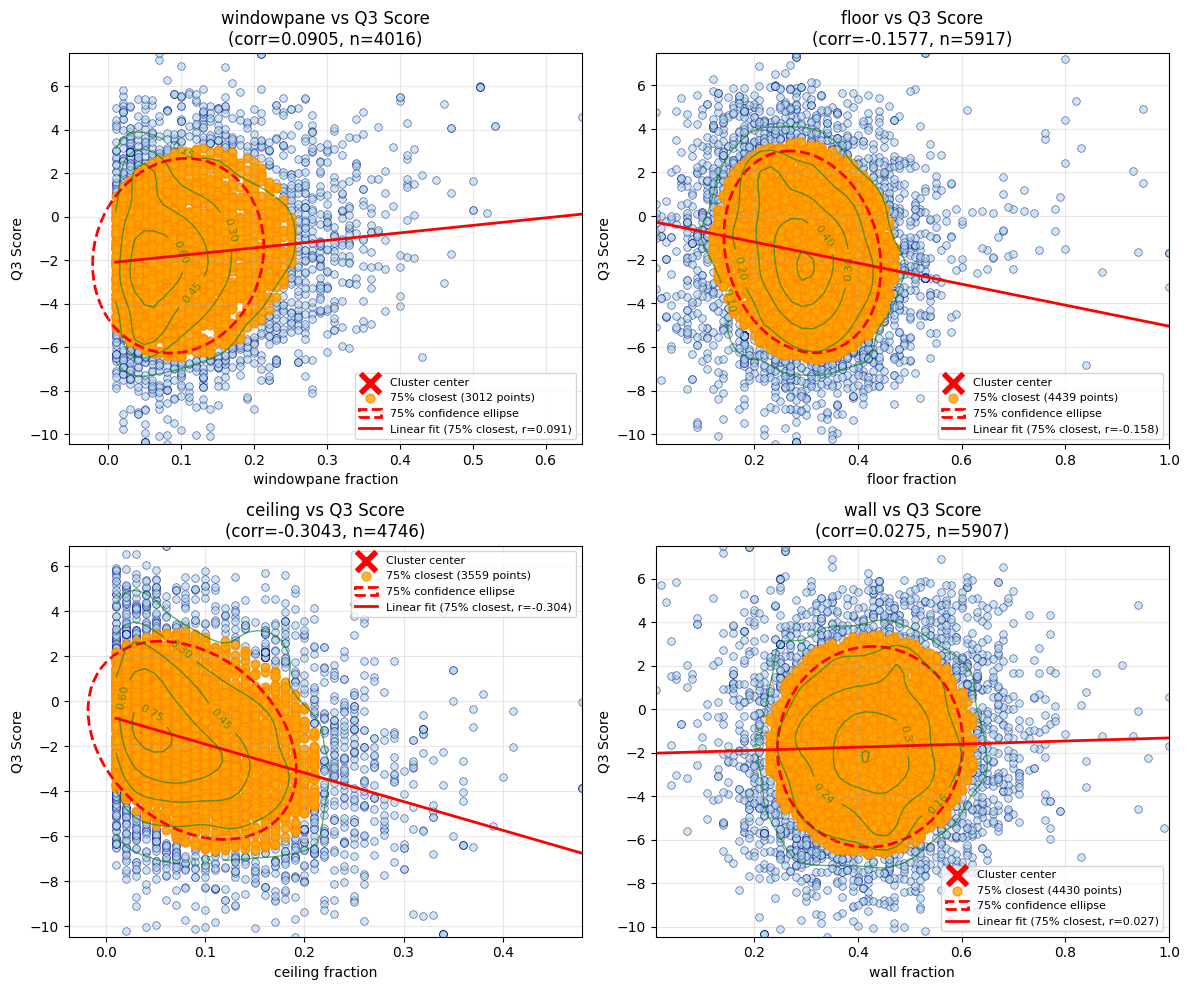
\includegraphics[width=0.8\columnwidth]{plots/inter_q3_cluster.png}
    \captionof{figure}{Cluster analysis of impression scores vs. interior element ratios}
    \label{fig:inter_q3_cluster}
\end{center}



% \subsection{Temporal Pattern Analysis}
% We also analyzed correlations between VGA statistics, interior segmentation results, and property data.
% Figure \ref{fig:q3_10years_box} shows q3 impression scores by construction decade, revealing trends in 
% perceived spatial quality over time. This demonstrates how our framework can identify temporal patterns 
% in housing design preferences.

% Additionally, Figure \ref{fig:pie_type} shows the distribution of property types in our dataset, 
% providing context for the composition of analyzed rental properties.

% \begin{flushleft}
%     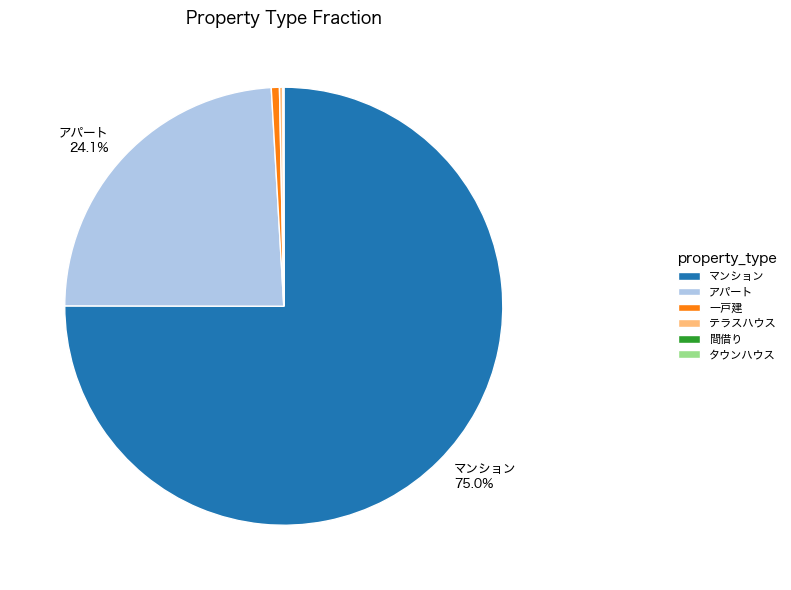
\includegraphics[width=0.7\columnwidth]{plots/pie_type.png}
%     \captionof{figure}{Distribution of property types in the analyzed dataset}
%     \label{fig:pie_type}
% \end{flushleft}

\subsection{Regression Analysis Against Rent Cost}
We performed regression analysis to predict rent cost using openness attributes. XGBoost achieved 
the best fit with acceptable $R^2$ scores. Analysis reveals that standard deviation and total sum 
of VGA values are the most important factors for rent prediction, thus there is a possibility 
that larger rooms with more spatial subdivisions tend to increase rental prices in a human understandable way.
The distance towards the top 2 stations falls behind the above factors slightly.
Additionally, our analysis reveals that user impression scores contribute to rent price trends moderately, 
suggesting a meaningful relationship between subjective spatial perception and market valuation. 
This indicates that user-perceived spatial quality aligns with economic value assessment in the rental market.
As shown in Figure \ref{fig:rent_regression}, training and testing results demonstrate reasonable performance. 
Residual analysis reveals weak bias in the fit, indicating the results are trustworthy. 

\begin{center}
    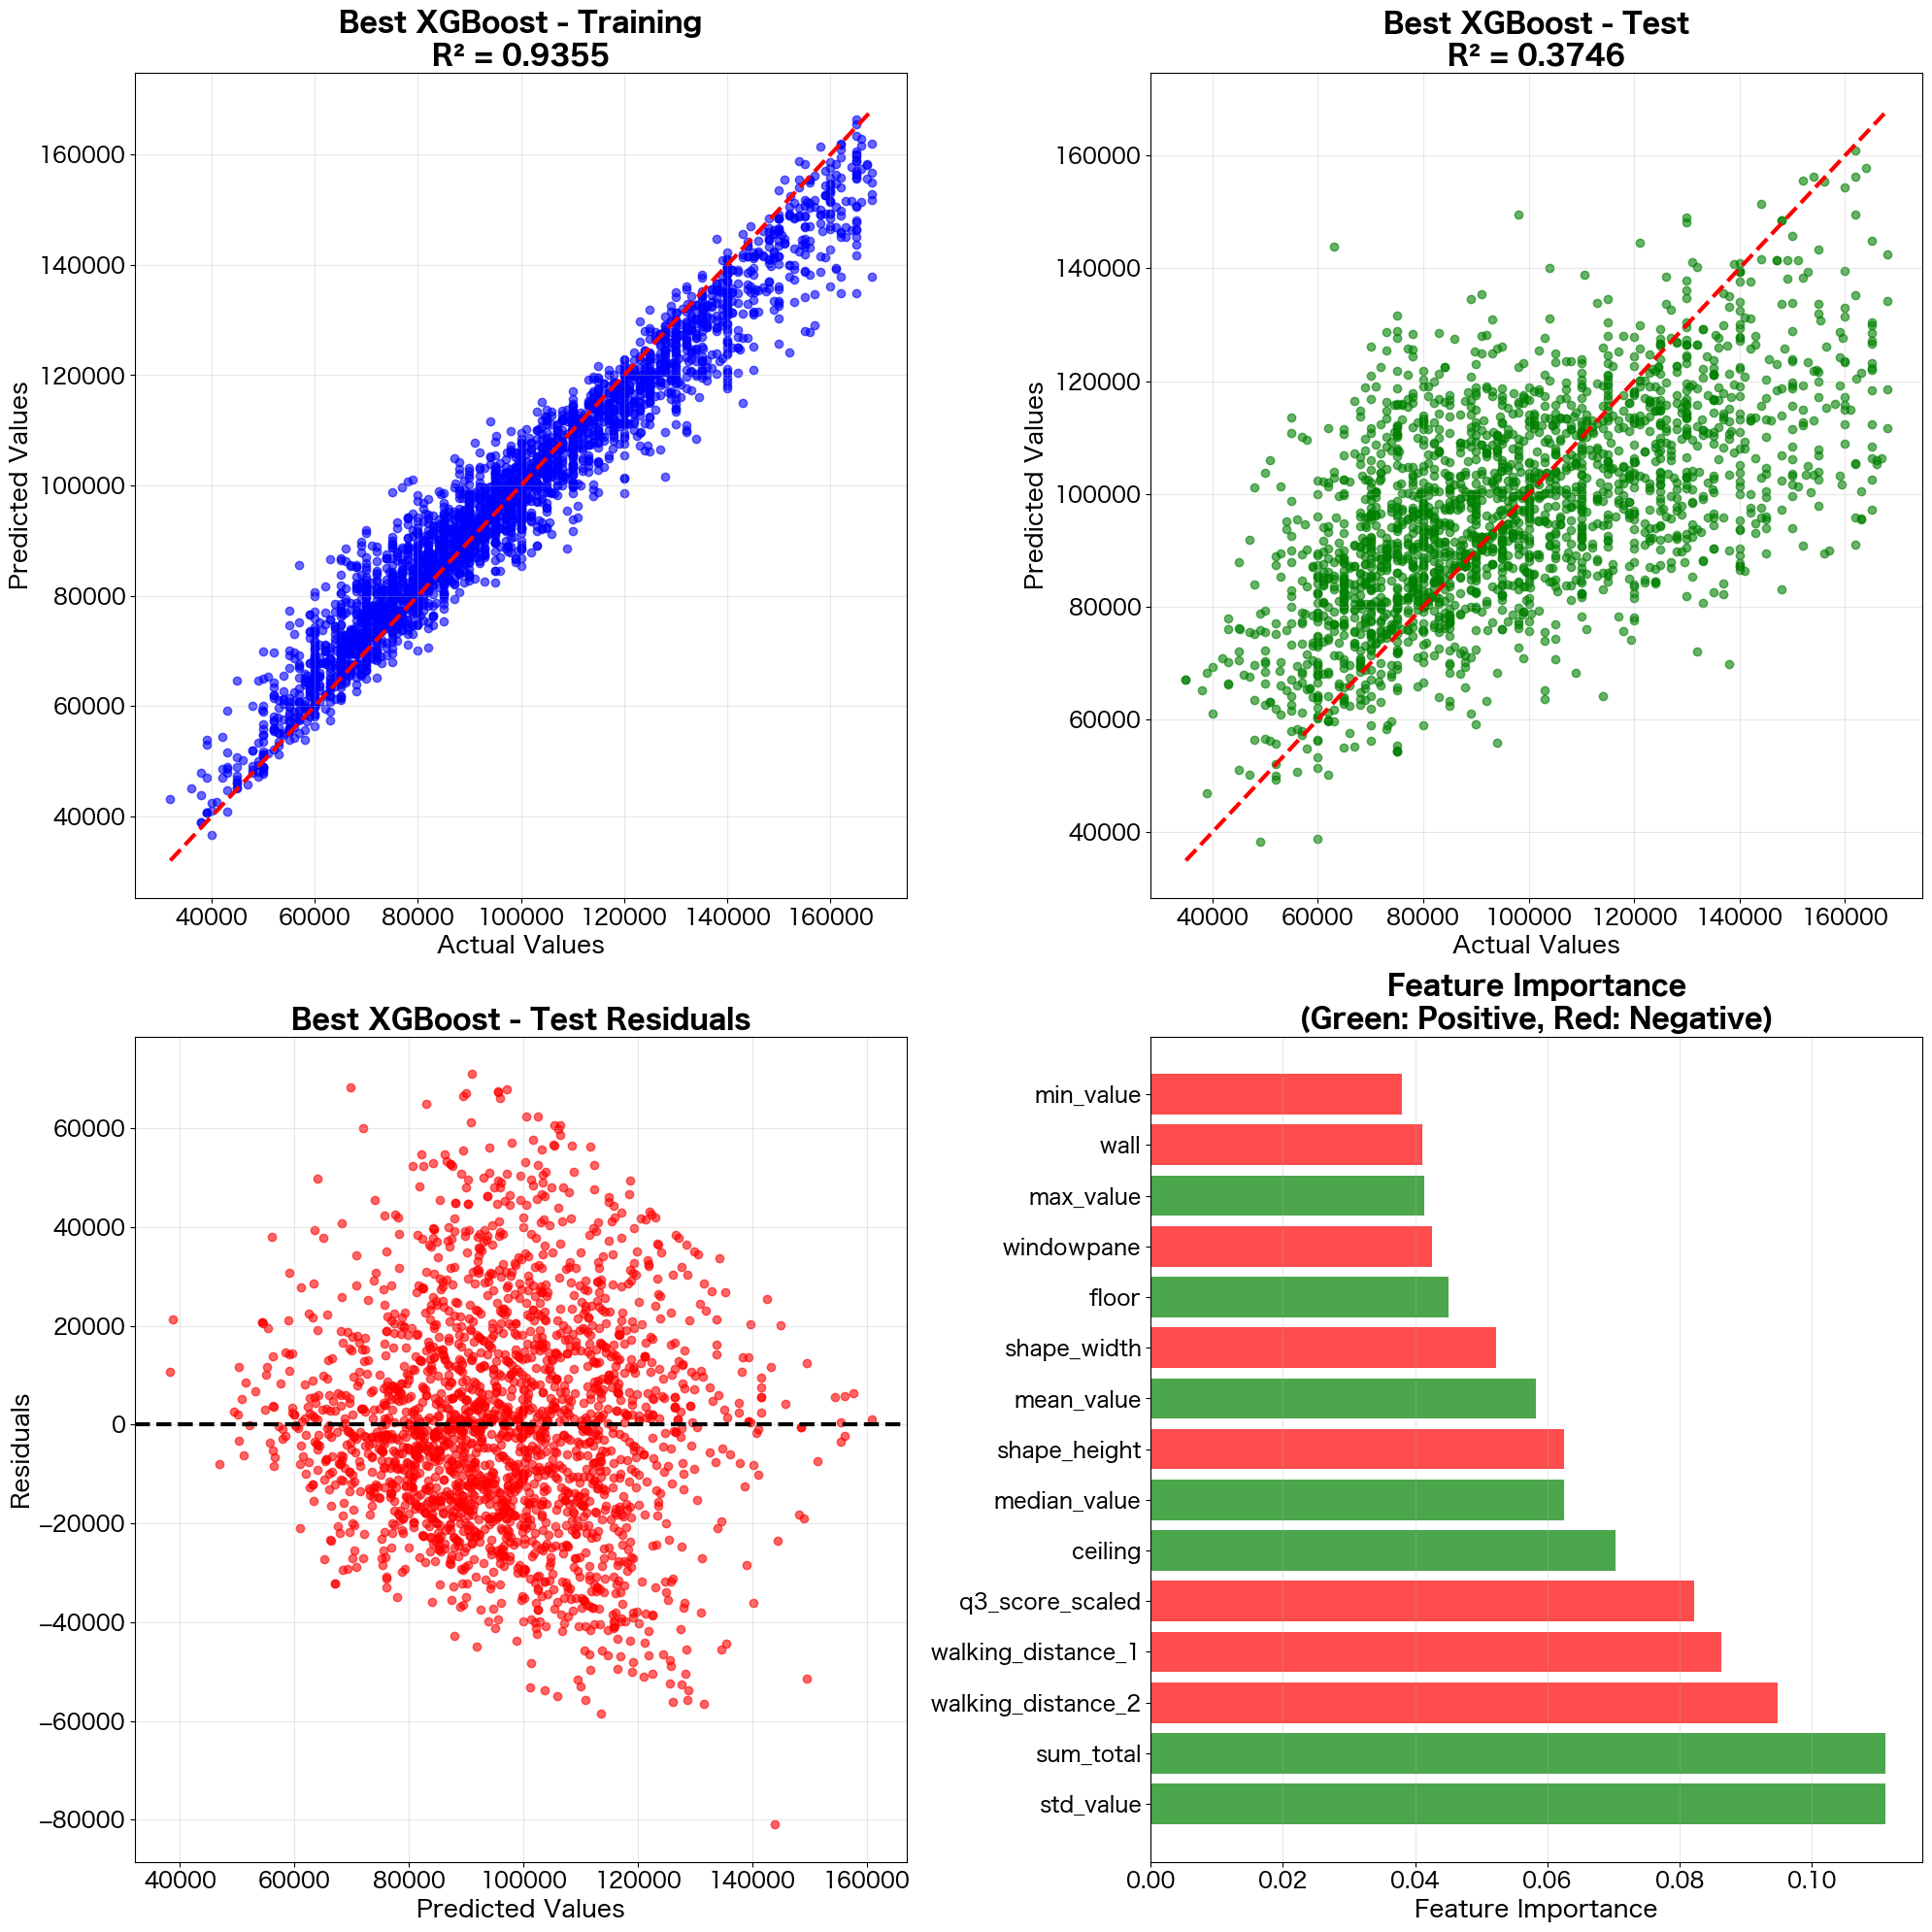
\includegraphics[width=0.75\columnwidth]{plots/rent_regression.png}
    \captionof{figure}{XGBoost regression results for rent prediction using openness attributes}
    \label{fig:rent_regression}
\end{center}


\subsection{Principal Component Analysis}
To better understand the relationships between spatial features, we performed Principal Component Analysis (PCA) 
using VGA mean values, ceiling, wall, floor, and window visual fractions as input features. The analysis reveals 
the underlying structure of spatial characteristics in our dataset. The PCA plots are shown as Figure \ref{fig:pca_dist}.
\begin{center}
    \begin{minipage}{0.45\columnwidth}
        \centering
        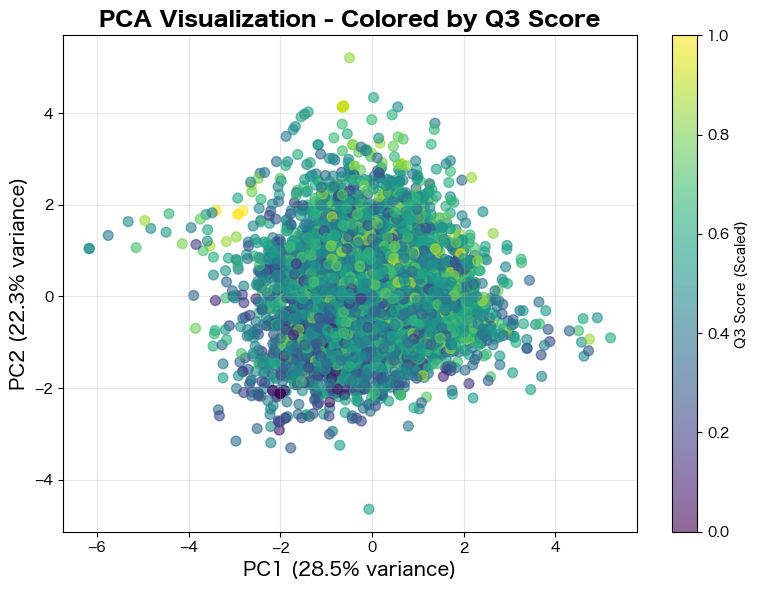
\includegraphics[width=\textwidth]{plots/PCA_01.png}
    \end{minipage}
    \hfill
    \begin{minipage}{0.45\columnwidth}
        \centering
        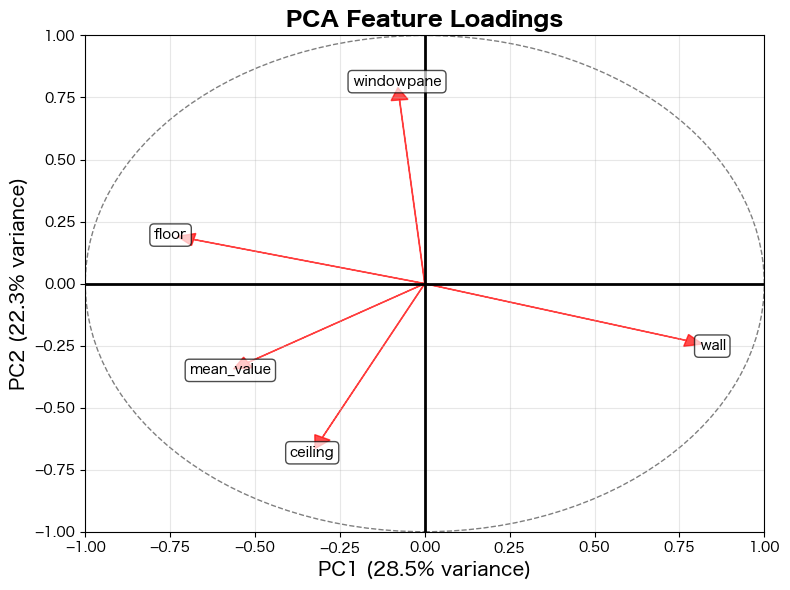
\includegraphics[width=\textwidth]{plots/PCA_02.png}
    \end{minipage}
    \captionof{figure}{PCA distribution and top 2 components with raw feature axis}
    \label{fig:pca_dist}
\end{center}


Table \ref{tab:pca_variance} presents the explained variance for each principal component. The first two 
components capture approximately 51\% of the total variance.
\begin{center}
\begin{tabular}{c|c|c|c}
\hline
Comp. & Eigenvalue & Var. \% & Cum. \% \\
\hline
PC1 & 1.42 & 28.46 & 28.46 \\
PC2 & 1.12 & 22.33 & 50.80 \\
PC3 & 1.07 & 21.36 & 72.16 \\
PC4 & 0.88 & 17.57 & 89.73 \\
PC5 & 0.51 & 10.27 & 100.00 \\
\hline
\end{tabular}
\captionof{table}{Principal component variance explanation}
\label{tab:pca_variance}
\end{center}
Table \ref{tab:pca_loadings} shows the feature loadings for all principal components. PC1 is primarily 
dominated by wall fractions (0.65) opposing floor visibility (-0.57). PC2 captures the balance between natural lighting (window: 0.70) 
and ceiling prominence (-0.59).

\begin{center}
\begin{tabular}{l|c|c|c|c|c}
\hline
Name & PC1 & PC2 & PC3 & PC4 & PC5 \\
\hline
VGA. Avg & -0.44 & -0.30 & -0.15 & 0.82 & -0.15 \\
Window & -0.06 & 0.70 & 0.50 & 0.37 & 0.35 \\
Floor & -0.57 & 0.17 & -0.53 & -0.23 & 0.56 \\
Ceiling & -0.25 & -0.59 & 0.62 & -0.16 & 0.43 \\
Wall & 0.65 & -0.22 & -0.27 & 0.32 & 0.60 \\
\hline
\end{tabular}
\captionof{table}{Principal component feature loadings}
\label{tab:pca_loadings}
\end{center}


\vspace{1em}

\section{Conclusions}

This research presents a framework for analyzing spatial openness in rental housing through automated madori
interpretation, visibility graph analysis, and interior semantic segmentation. Our methodology quantifies subjective 
spatial qualities using visual data from rental platforms. Key findings reveal weak correlations between VGA metrics 
and user impression scores, with excessive floor/ceiling visibility negatively impacting quality perceptions. 
PCA analysis reveals that the first two components capture 51\% of variance, with PC1 dominated by wall-floor 
opposition and PC2 capturing natural lighting versus ceiling prominence. Regression analysis demonstrates that VGA 
standard deviation and room size are the most important factors for rent prediction. Spatial openness perception is 
impacted by the complex interactions between these factors. Our results identify their distinct contributions, 
revealing how visual effects and VGA metrics shape openness evaluation. This research provides practical tools for 
data-driven spatial openness analysis, which is a step towards openness-oriented housing design.

% \section{References}

% [References would be listed here.]

\end{multicols}

\newpage

\begin{multicols}{2}
\fontsize{11}{11}\selectfont

% Additional content for page 3 would continue here
% This could include detailed methodology descriptions,
% additional results, or extended discussion sections

\end{multicols}

\newpage

\begin{multicols}{2}
\fontsize{11}{13}\selectfont

% Final page content would be placed here
% This might include appendices, additional references,
% or supplementary analysis results

\end{multicols}

\end{document}